\documentclass{article}


% if you need to pass options to natbib, use, e.g.:
%     \PassOptionsToPackage{numbers, compress}{natbib}
% before loading neurips_2023


% ready for submission
\usepackage[final]{neurips_2023}


% to compile a preprint version, e.g., for submission to arXiv, add add the
% [preprint] option:
%     \usepackage[preprint]{neurips_2023}


% to compile a camera-ready version, add the [final] option, e.g.:
%     \usepackage[final]{neurips_2023}


% to avoid loading the natbib package, add option nonatbib:
%    \usepackage[nonatbib]{neurips_2023}


\usepackage[utf8]{inputenc} % allow utf-8 input
\usepackage[T1]{fontenc}    % use 8-bit T1 fonts
\usepackage{hyperref}       % hyperlinks
\usepackage{url}            % simple URL typesetting
\usepackage{booktabs}       % professional-quality tables
\usepackage{amsfonts}       % blackboard math symbols
\usepackage{nicefrac}       % compact symbols for 1/2, etc.
\usepackage{microtype}      % microtypography
\usepackage{xcolor}         % colors
\usepackage{graphicx}

% Title ideas: 
% A Blind Approach to Hyperspectral Deep Deconvolution
% Deep Learning for Hyperspectral Blind Deconvolution
% Deep Learning for Hyperspectral Deconvolution
% Hyperspectral Blind Deep Deconvolution
% Blind Deep Deconvolution for Snapshot Hyperspectral Images
% Deep Blind Deconvolution for Snapshot Hyperspectral Images
\title{Hyperspectral Deep Deconvolution}

\author{%
   Corey Zheng \\
   College of Biomedical Engineering, Georgia Tech  \\
  % Address \\
   \texttt{czheng@gatech.edu} \\
   \AND
   Austin Barton \\
   Georgia Tech \\
  % Address \\
   \texttt{abarton40@gatech.edu} \\
   \And
   Mohammad Taher \\
   Georgia Tech \\
  % Address \\
   \texttt{mtaher3@gatech.edu} \\
   \And
   Memesh Abdulaziz \\
   Georgia Tech \\
  % Address \\
   \texttt{a.memesh@gatech.edu} \\
}


\begin{document}

\maketitle


\begin{abstract}
  This paper addresses the challenge of chromatic aberration in snapshot hyperspectral imaging, where the introduction of a third spectral dimension complicates encoding information into a two-dimensional detector plane. While traditional methods rely on scan-based approaches, our proposed method aims to enhance the quality of hyperspectral images by mitigating distortions inherent in snapshot acquisitions by leveraging a blind deconvolution approach with a U-Net neural network architecture. Our approach allows real-time correction without the need for complex scanning mechanisms nor knowledge of point spread functions. Through experimental validation, we demonstrate the efficacy of our method in preserving image structure and chemical composition information contributing to improved imaging throughput and simplified hardware requirements. Our paper represents a simple yet effective approach to circumventing blurring issues in snapshot hyperspectral imaging, providing a practical solution for applications in medical imaging, agriculture, materials identification, and geological surveillance.
\end{abstract}


\section{Introduction}
Hyperspectral imaging is a highly important imaging modality, with the ability to capture the unique wavelength emission and reflectance spectra of objects within the field of view. For every spatial pixel within a hyperspectral image, the captured spectrum is a superposition of all unique spectra produced by molecules within the spatial region, and thus is a measure of the chemical composition at each spatial location within the field of view (FOV). This higher-dimensional spectral information has therefore enabled major strides in medical imaging \cite{lu2014medical}, agriculture \cite{lu2020recent}, materials identification \cite{dong2019review}, geological surveillance \cite{peyghambari2021hyperspectral}, and more.  

However, hyperspectral images have been difficult to acquire, as their three-dimensional nature (two spatial dimensions and a spectral dimension) cannot be fully represented on electronic image sensors which feature two-dimensional arrays of pixels. As a result, traditional hyperspectral imaging approaches are scan-based, scanning through either one spatial dimension such as pushbroom approaches, or one spectral dimension by utilizing a series of filters \cite{gao2015optical}. Such approaches limit the imaging throughput speed and also require more complex imaging setups that involving parts such as scanning galvo mirrors, acousto-optical deflectors, filters, or acousto-optical filters.

In contrast, \textit{snapshot} hyperspectral imaging seeks to capture both the full spectrum and spatial information in a single image frame, greatly increasing the acquisition throughput. Furthermore, these imaging systems can be implemented with static hardware as opposed to traditional methods that require actively modulated optical components to produce scanning motions. However, it is challenging to encode this higher dimensional information seamlessly into the two-dimensional detector plane. 

Early snapshot hyperspectral imaging began by mapping slices of the hyperspectral volume to different spatial positions on a two-dimensional camera detector. Approaches in this category include Computed Tomography Imaging Spectrometers (CTIS), which projects an array (7×7) of tiled image copies, and Integral Field Spectrography (IFS) which disperses image slices via prism, elongating the area the image occupies on the sensor. These mapping approaches necessitate a trade-off by reducing either the field of view (FOV) or volume in order to fit both the spatial image and spectral components onto a sensor with the same number of pixels.

Motivated by this inherent compromise, various computational based approaches aimed at reconstructing the hyperspectral information without sub-image divisions have been introduced. In particular, \textit{chromatic aberration} approaches  


As a result, true single-image snapshot hyperspectral imaging approaches have been attempted. A major challenge with these approaches however, is the very ill-posed problem of restoring a hyperspectral stack from a monochromatic image comprised of the superposition of different chromatic blur kernels. 

Our goal will be to perform similar snapshot hyperspectral imaging, but utilizing customary achromatic optics, which are common off-the-shelf components. We will utilize deep learning to form the reconstruction process.


\section{Related Works}
In this section we review approaches towards hyperspectral snapshot imaging.

\subsection{CTIS}
Snapshot hyperspectral imaging began with the introduction of Computed Tomography Imaging Spectrometers (CTIS) \cite{FORD2001986}. In this approach, an additional dispersive element is introduced into the imaging system, essentially splitting an incoming image into multiple tiled copies, with each copy exhibiting a different amount of radial chromatic blur. This follows the same concept as lightfield imaging \cite{guo2019fourier}\cite{broxton2013wave} but utilizes diffraction orders produced from chromaticity rather than depth. In a sense, such an approach could also be considered a class of \textit{chromatic aberration} approaches. However, it is differentiated from other chromatic aberration approaches by key disadvantages: (1) The authors utilize an iterative reconstruction algorithm (MART) in order to recover the final image, but this algorithm is time consuming and requires measurement of multiple calibration matrices. (2) The usage of a dispersive element to create multiple tiled copies (e.g. 7×7) results in a reduction in the field of view of the image, since the camera sensor is split up into smaller images.

\subsection{Bioinspired Chromatic Vision Blur}
Unlike mammalian eyes which have separate neuroreceptors with sensitivities tailored towards different wavelengths (primarily red, blue, green), cephalopod eyes have broadband neuroreceptors sensitive to all wavelengths. Yet, these animals can still discriminate colors through recognition of the form of the chromatic blur they produce. Inspired by this, Zhan et al. utilized a chromatic aberration system coupled with an SVD-based iterative reconstruction algorithm to restore hyperspectral stacks from monochromatic blurred images \cite{zhan2019hyperspectral}. However, the authors had to utilize 3 images of the same object at different distances in order to achieve their results. Furthermore, the data the authors demonstrated their results on was extremely well-behaved simulation data - the authors only showed reconstruction on images that contained single-peak gaussian-esq spectra, rather than more realistic scenarios, indicating that there may have been potential trouble with separability in their approach.

\subsection{Diffracted Rotation}
Utilizing dispersion engineering, it is possible to create custom optical elements with controllable chromatic blurring patterns. Jeon et al. \cite{jeon2019compact} formulated an approach, designing a custom diffractive optical element (DOE) that creates a triple-helix point-spread function which rotates based on the wavelength. Thus, the authors were able to increase the separability of the chromatically-aberrated images by eliminating the radial symmetry of their blur kernels. They combined this with a learned unrolled network architecture based on U-net, combined with an iterative algorithm to reconstruct hyperspectral stacks. Though their approach appears quite successful, it requires a custom optical element which is difficult to manufacture.

\section{Methods}

\subsection{Inputs and Outputs}

The input is a 1x128x128 pixel greyscale image captured from a monochromatic sensor with uniform sensitivity across all channels. The output is a 29x128x128 set of images representing the expected outcome of using all possible 29 PSFs.

\subsection{Image formation model}

Our project revolves around the idea of induced chromatic aberration leading to known blurring patterns dependent on wavelengths which can be separated utilizing our deep-learning algorithm. As a brief background, the blur kernel, or point spread function (PSF) is the impulse response of an imaging system, or the blur associated with imaging an infinitesimal point source. Such example PSFs are illustrated in the top of Figure \ref{fig:data}. As a basis for the optical physics of the system, our image formation model utilizes the following assumptions:
\begin{enumerate}
    \item The PSF is \textit{spatially invariant}: the shape of the PSF is not dependent on the spatial location of the objects in the image.
    \item The camera operates in the \textit{hyperfocal range}: the camera sensor is placed at the focal point of the optical lens, and all objects imaged by the camera are at a far enough distance $>H$ that they can be considered at infinity, where $H$ is defined as:
    \begin{equation}
        H \approx \frac{f^2}{Nc}
    \end{equation}
    Where $H$ is the hyperfocal distance, $f$ is the focal length of the lens, $N$ is the F-number, and $c$ is the diffraction-limited spot size. This assumption is important as it constrains the degrees of freedom of our PSF. Under this assumption, the shape of the PSF is to be solely dependent on wavelength; i.e., $PSF(\lambda)$ instead of both wavelength and depth ($PSF(\lambda,z)$).
    \item The camera has uniform sensitivity across the entire light spectrum.
\end{enumerate}

Assumption (1) is frequently utilized in optical imaging fields, as with it an image can be conveniently described as the convolution of an underlying object with the PSF:

\begin{equation}
    I(\lambda) = g(\lambda) \ast PSF(\lambda)
\end{equation}

Where $I(\lambda)$ is the captured image at some wavelength and $g(\lambda)$ is the underlying unblurred object at some wavelength. Given that the imaging camera has no filters and captures all wavelengths equally via assumption (3), the image produced will thus be:

\begin{equation}
    I = \int_\lambda g(\lambda) \ast PSF(\lambda)
\end{equation}

Whilst this may seem like a highly constraining set of assumptions, these are often employed in optical imaging to simplify the computational process, being similarly applied in a related work \cite{jeon2019compact}. This is the image formation model upon which we build our dataset described in a further section.

\section{Blind Deconvolution Using a U-Net}

\subsection{U-Net}
To solve this task, we're using the U-Net model, a deep convolutional neural network model developed for biomedical image segmentation by Ronneberger et al. \cite{Ronneberger_2018}. In their paper, they discuss one of the defining characteristics of their task was the fact that the desired output required localization, i.e. each pixel value outputted is measured against a target value. Their U-Net outperformed the existing method of patchwise classification via CNNs and drastically improved the computational costs in achieving their task as compared to other existing methods at that time. The architecture consists of a contracting path to capture context and a symmetric expanding path that enables precise localization, similar to an autoencoder for two-dimensional input data but with skip connections from the encoded representations of the input to the decoded outputs at each upsampling step. The model will be implemented using PyTorch with the structure referenced in Figure \ref{fig:Unet_model}.   

\subsection{Objective Function}
Our conceptual objective is to minimize the difference of the spectral information as well as perceptual quality between the output and ground truth images. Therefore, the objective functions we experiment with are Structural Similarity Index Measure (SSIM) and Mean Squared Error (MSE). SSIM is a common metric for image comparisons that compares the overall shapes and patterns, while MSE focuses on the raw pixel value differences \cite{Brunet_Vrscay_Wang_2011}.

An underlying issue that MSE, and other similar loss functions, have in the context of image restoration is the fact that many perceptually different restored images can correspond to one MSE value. Because our problem is taking hyperspectral images that are corrupted by chromatic aberration and restoring them to their corresponding latent sharp images, it is possible that deblurred images outputted by our model may have low MSE but perceptually poor quality.

SSIM achieves accurate image comparisons without allowing the overall structure of the image to change, so the network can't recreate an image that's completely different. This metric's goal is to accurately measure the perceptual quality of an image using a combination similarity
measurements between each image's luminance, contrast, and structure. Luminance is described by a function of each image's the mean pixel value, contrast is described by a function of each image's standard deviation, and structure is a function of the centered and normalized pixel values. Something important to note is that the range of SSIM is $[-1, 1]$ with larger output values corresponding to greater similarity. Therefore, we formulate our "SSIM Loss" function as
\begin{equation}
    \texttt{SSIM}_{Loss} = 1 - \texttt{SSIM}
\end{equation}

which has a range of $[0, 2]$, with high similarity corresponding to lower values. However, this may cause the model to prioritize improving structural similarity to the point where it fails to restore spectral information. On the other hand, MSE can severely penalize any pixel differences, which may ensure that we don't lose as much information, specifically spectral information. 

We experimented with a combination of both of these since our problem requires both image deblurring and spectral information recovering.

\section{Data Processing}
\subsection{Dataset}
We are utilizing a combination of 5 hyperspectral datasets \cite{CAVE_0293}\cite{chakrabarti2011statistics}\cite{arad_and_ben_shahar_2016_ECCV}\cite{DeepCASSI:SIGA:2017}\cite{farrell2003simulation}, which results in a total of 394 unique hyperspectral images covering objects including human faces, architecture, household objects, landscapes, and more.


\subsection{Data Preprocessing}
Because the 5 hyperspectral datasets we collected utilized different wavelength ranges, we cropped out only the spectral ranges that every dataset had in common (420-700nm in steps of 10nm). This formed our ground truth set. In order to generate our input data, we had to simulate what it would look like if the image was captured by a chromatically-blurring imaging system. We first resized each image, keeping the aspect ratio, to the same height of 512px. This is because some images were taken with very high resolutions (4K or greater) and because we are using a patch-generation strategy, we wanted to keep the feature density of each image high and minimize the chances of sampling empty or very low-feature patches. Afterwards described previously, we performed a convolution with the hyperspectral PSF as described in the image formation model to generate a monochromatic blurred image, depicted in the flowchart of Figure \ref{fig:data_pipeline}. Finally, we randomly sampled 16 128×128 pixel patches from each image and extracted the corresponding 128×128×29 pixel hyperspectral volume to form input and output pairs, respectively.

In total, we have 6304 patches, without considering augmentations. We will first determine the performance of the model without augmentation. If this does not work well, we will apply augmentation, specifically flipping and resizing. Considering the initial resizing of all images to 512 pixels, there is significant potential for multi-scale augmentations and combined with rotations and flipping, we could greatly increase the dataset by at least an order of magnitude. The drawback is that these augmentations must be applied prior to PSF convolution (due to an asymmetric PSF and scale dependence), which would increase the already-large datasets representation on disk.

\begin{figure}
  \centering
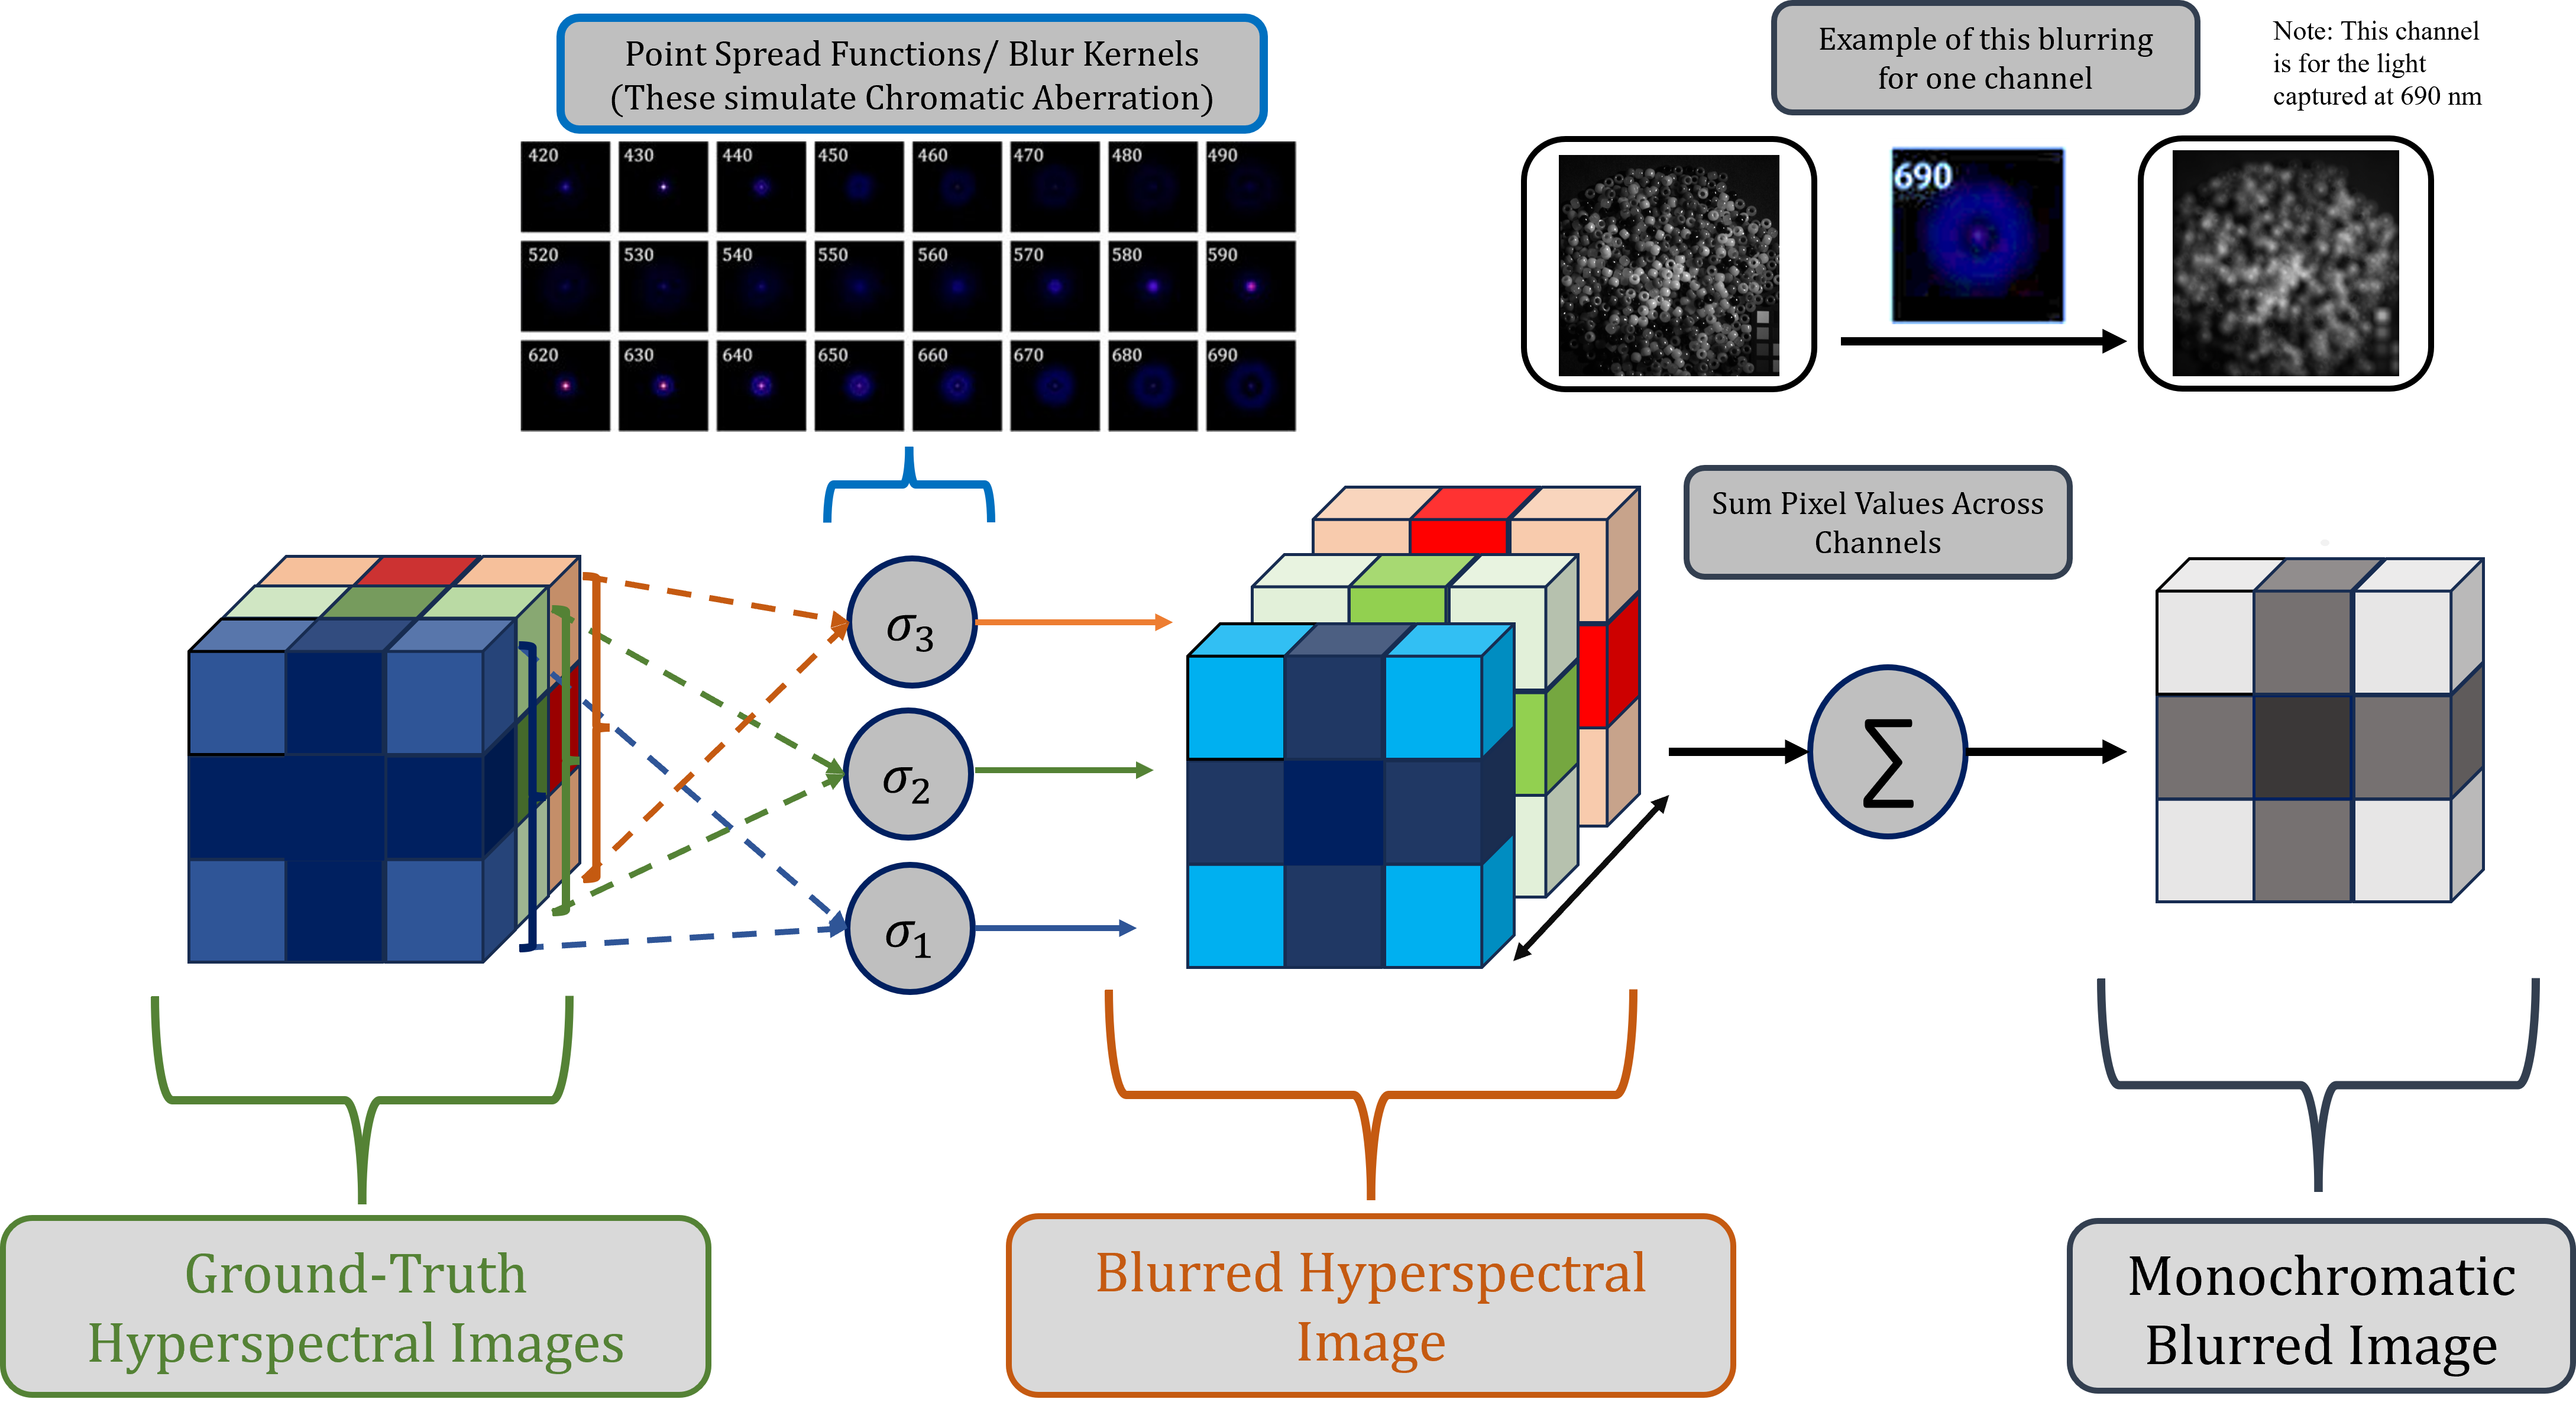
\includegraphics[width=\textwidth]{figs/data_synthesization/simulate_data_pipeline.png}
  \caption{Data Synthesization Pipeline.}
  \label{fig:data_pipeline}
\end{figure}

\section{Results}

\begin{figure}[!h]
    \centering
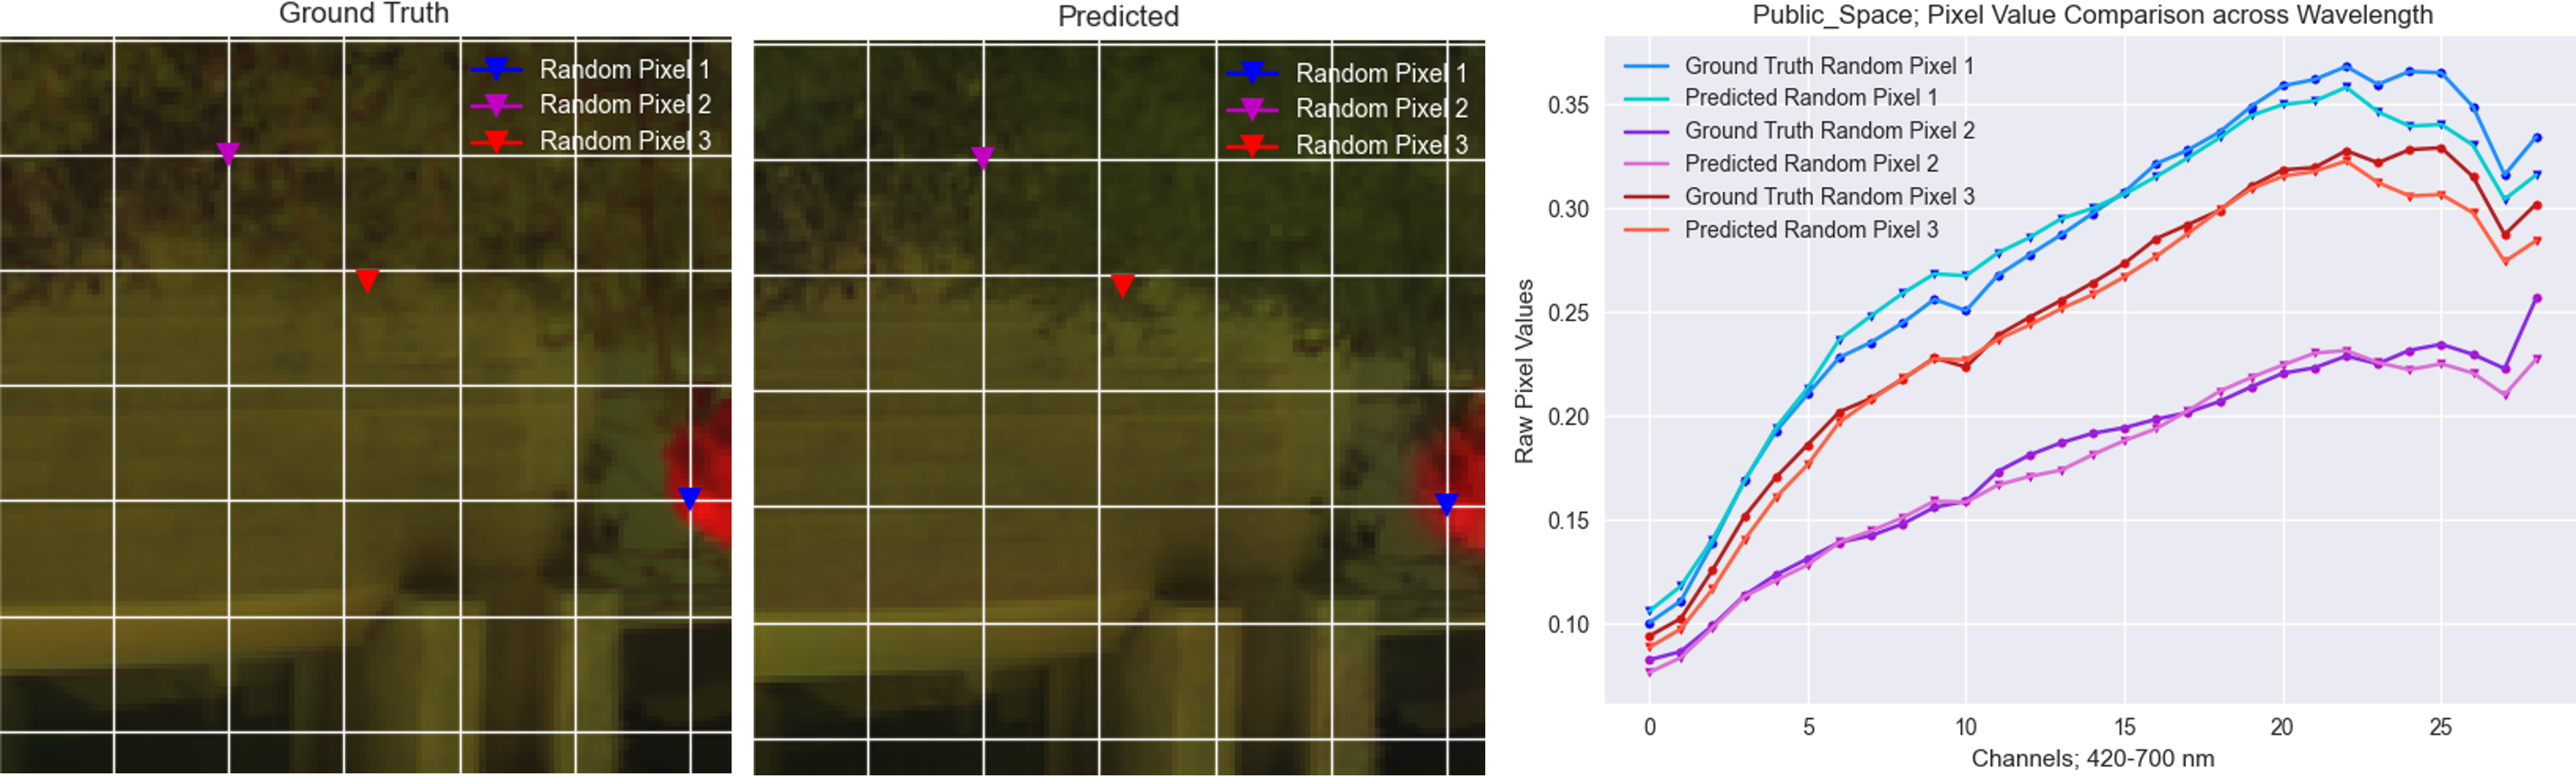
\includegraphics[width=\textwidth]{figs/ClassicUnet/pixel_comparison/PublicSpaceConsolidated.png}
    \caption{Test Sample Pixel Comparison between Ground Truth and Predicted Images for Classic U-Net.}
    \label{fig:PublicSpacePC}
\end{figure}

\iffalse
\section*{References}


References follow the acknowledgments in the camera-ready paper. Use unnumbered first-level heading for
the references. Any choice of citation style is acceptable as long as you are
consistent. It is permissible to reduce the font size to \verb+small+ (9 point)
when listing the references.
Note that the Reference section does not count towards the page limit.
\medskip


{
\small


[1] Alexander, J.A.\ \& Mozer, M.C.\ (1995) Template-based algorithms for
connectionist rule extraction. In G.\ Tesauro, D.S.\ Touretzky and T.K.\ Leen
(eds.), {\it Advances in Neural Information Processing Systems 7},
pp.\ 609--616. Cambridge, MA: MIT Press.


[2] Bower, J.M.\ \& Beeman, D.\ (1995) {\it The Book of GENESIS: Exploring
  Realistic Neural Models with the GEneral NEural SImulation System.}  New York:
TELOS/Springer--Verlag.


[3] Hasselmo, M.E., Schnell, E.\ \& Barkai, E.\ (1995) Dynamics of learning and
recall at excitatory recurrent synapses and cholinergic modulation in rat
hippocampal region CA3. {\it Journal of Neuroscience} {\bf 15}(7):5249-5262.
}
\fi

%%%%%%%%%%%%%%%%%%%%%%%%%%%%%%%%%%%%%%%%%%%%%%%%%%%%%%%%%%%%
\bibliographystyle{plainnat}
\bibliography{paper/ref}

\newpage

\section{Supplementary Material}

\begin{figure}[!htb]
    \centering
    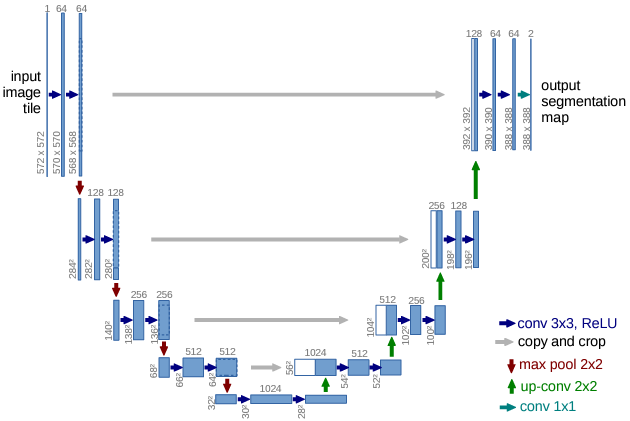
\includegraphics[width=\textwidth]{figs/model/UNet_model.png}
    \caption{U-Net Architecture \cite{ronneberger2015u}}
    \label{fig:Unet_model}
\end{figure}


\end{document}